
\centering
\def\yshiftLabels{-0.7cm}
\def\distancePlotLabel{8.5cm}
\def\lineLength{13.3cm}
\def\heightplots{5.0cm}
\def\shortenLine{0.15cm}
\begin{tikzpicture}[thick]

%%%%%%%%%%%%%%%%%%%%%%%%%%%%%%%%%%%%%%%%%%%%%%%%%%%%%%%%%%%%
%%%%%%%%%%%%  Code             %%%%%%%%%%%%%%%%%%%%%%%%%%%%%
%%%%%%%%%%%%%%%%%%%%%%%%%%%%%%%%%%%%%%%%%%%%%%%%%%%%%%%%%%%%

  %%%%%%%%%%%%%%%%%%%
  %%%%%  Nodes  %%%%%
  %%%%%%%%%%%%%%%%%%%

%%%%%%% (a) Data %%%%%%% 
\node(data){
\tiny\begin{lstlisting}[mathescape, language=Venture, escapeinside={(*@}{@*)}]
define f = (x) -> {0.3 + 0.4*x + 0.5*sin(2.7*x) + 1.1/(1 + x**2)};
define N = 20;
define data_xs = mapv((_) -> {normal(0,1)}, arange(N));
define data_ys = mapv((x) -> {
    if(flip(0.95))
      {normal(f(x),0.1)}
    else
      {normal(f(x),1.0)}}, 
  data_xs);
define data = to_dict(zip(data_xs, data_ys));
assume look_up_function = (x_value) -> {(*@\$@*){data}[x_value]};
\end{lstlisting}};
\node[left=0.0cm of data.north west, yshift=\yshiftLabels] (a) {(a)};

%%%%%%% (b) Model %%%%%%% 
\node[below=1.52cm of data.south west, anchor=west] (model){
\tiny\begin{lstlisting}[mathescape, escapeinside={(*@}{@*)}]
assume scale_factor_log_odds_space $\sim$ log_odds_uniform() #hyperparameter:0;
assume lengthscale_log_odds_space $\sim$ log_odds_uniform() #hyperparameter:1;
assume scale_factor = -log_logistic(scale_factor_log_odds_space);
assume lengthscale =  -log_logistic(lengthscale_log_odds_space);
assume k_constant = gp_cov_const(1);
assume k_se = gp_cov_scale(scale_factor, gp_cov_se(lengthscale));
assume k_noise = gp_cov_scale(0.1, gp_cov_bump(0.0000001, 0.000001));
assume composite_covariance = gp_cov_sum(k_noise, 
  gp_cov_sum(k_se, k_constant));
assume gpmem = allocate_gpmem()(look_up_function, gp_mean_const(0), composite_covariance);
assume noisy_observation = mem((x) -> {
  latent_function_value $\sim$ gpmem[1]([x]) #latent_function_values:x;
  student_t(19, latent_function_value[0], 0.1)});
\end{lstlisting}};
\node[left=0.0cm of model.north west, yshift=\yshiftLabels] (b) {(b)};

%%%%%%% (c) observations %%%%%%% 
\node[below=0.2cm of model.south west, anchor=west] (observations) {
\tiny\begin{lstlisting}[mathescape, escapeinside={(*@}{@*)}]
for_each(arange(size(data_xs)), (i) -> {
  observe noisy_observation((*@\$@*){data_xs[i]}) = data_ys[i]});
\end{lstlisting}};
\node[left=0.0cm of observations.north west, yshift=\yshiftLabels] (c) {(c)};

%%%%%%% (d) inference %%%%%%% 
\node[below=0.3cm of observations.south west, anchor=west] (inference) {
\tiny\begin{lstlisting}[mathescape, escapeinside={(*@}{@*)}]
mh(minimal_subproblem(random_singleton(/?latent_function_values)), 500);
grad_ascent(minimal_subproblem(/?hyperparameter), 0.2, 1, 20);
mh(minimal_subproblem(random_singleton(/?hyperparameter)), 1);
\end{lstlisting}};
\node[left=0.0cm of inference.north west, yshift=\yshiftLabels] (d) {(d)};

%%%%%%% (e,f) inference walk %%%%%%% 
\node[below=3.1cm of inference.west, anchor=west, xshift=-0.55cm] (gradient_walk) {
  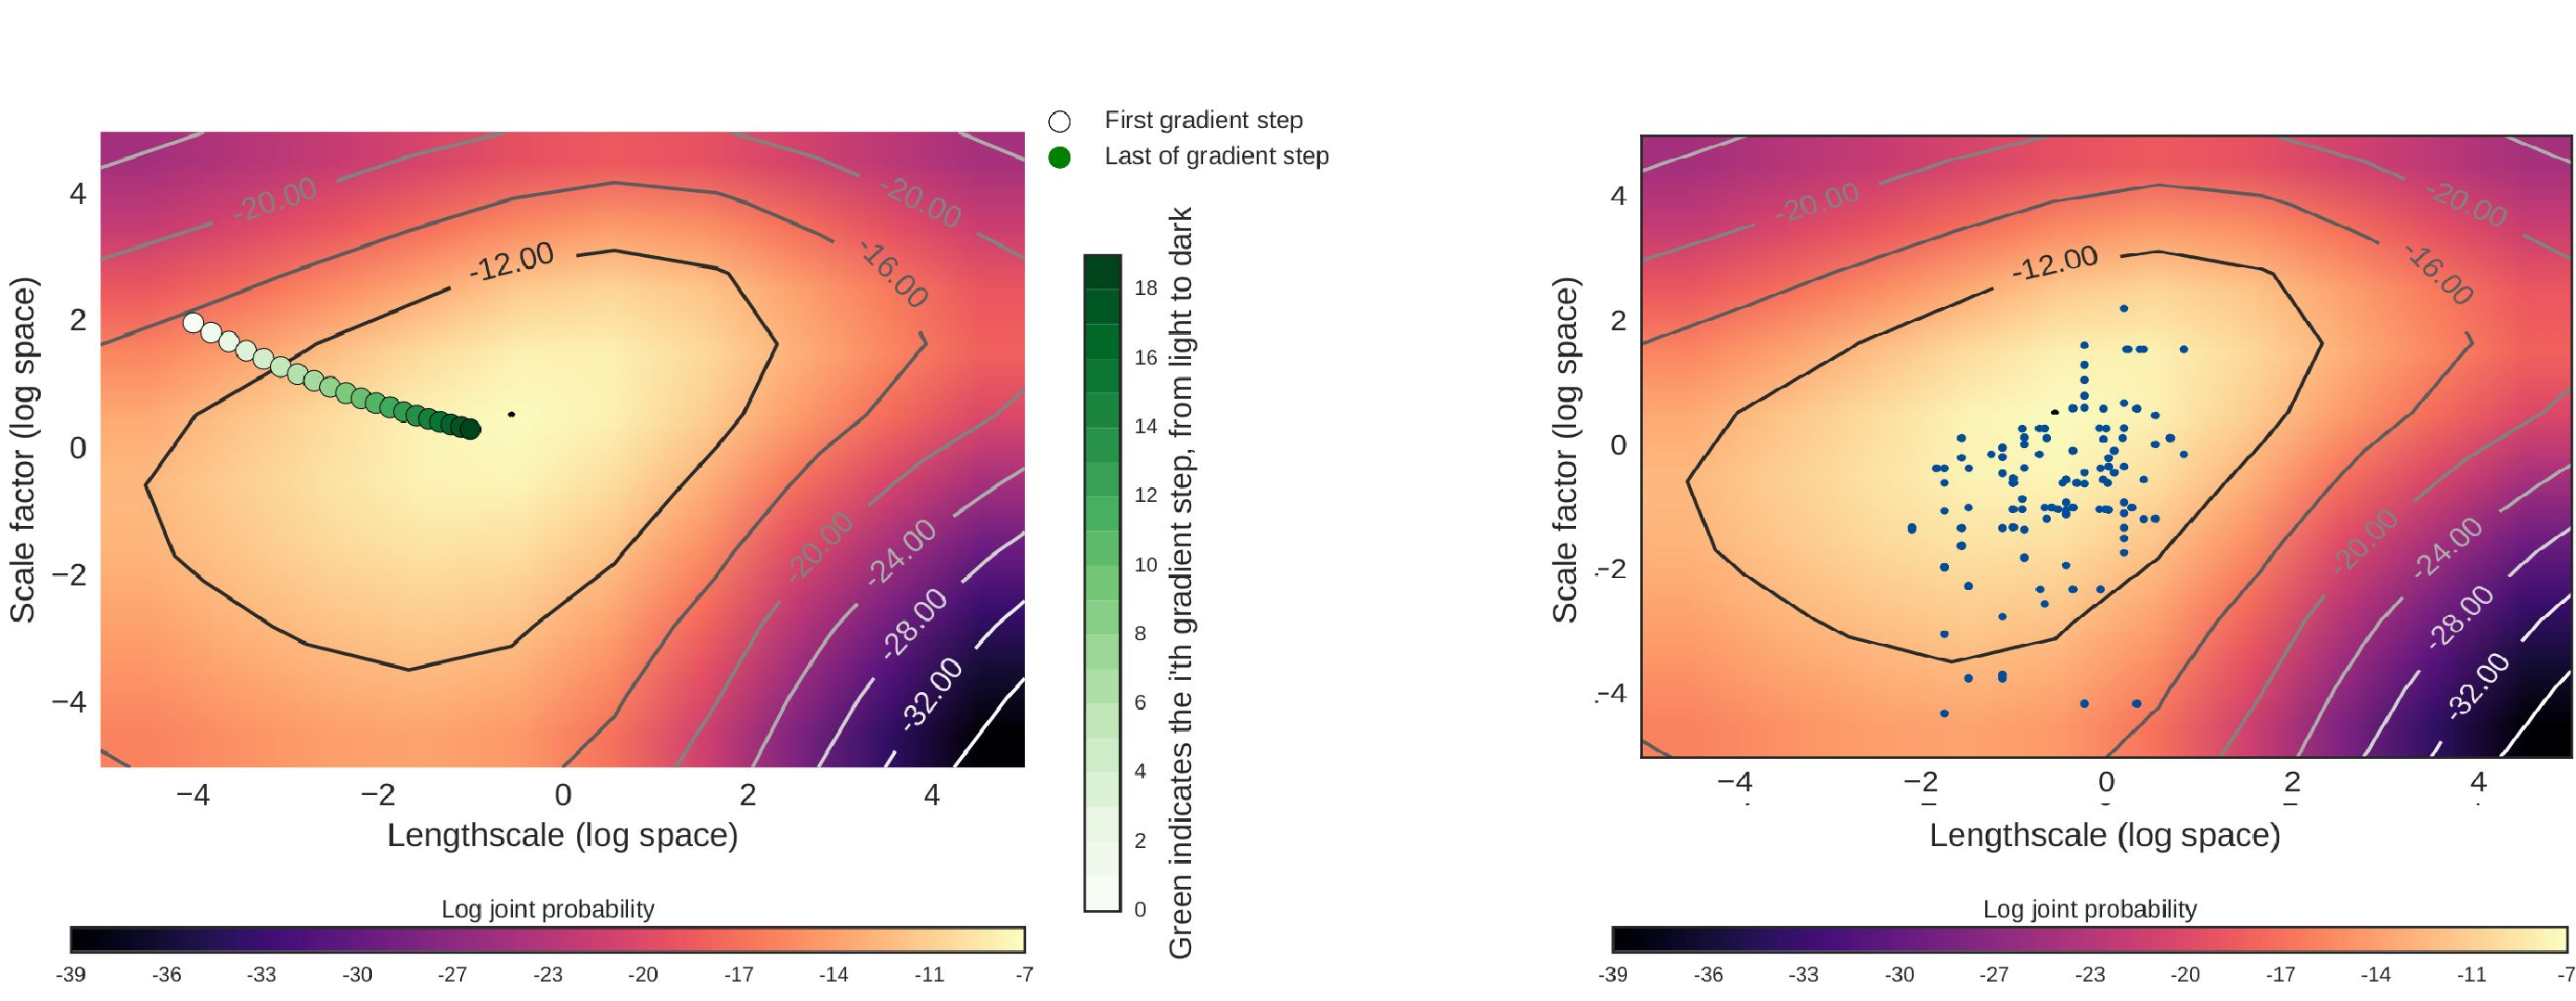
\includegraphics[width=0.85\textwidth]{figs/revised_figures/neal/neal_inference.pdf}
};
\node[left=-0.5cm of gradient_walk.north west, yshift=-0.5cm] (e) {(e)};
\node[right=7.0cm of e, yshift=0.0cm] (f) {(f)};
\node[right=0.3cm of e, yshift=0.0cm] (e_titel) {\footnotesize Trajectory of
gradient ascent};
\node[right=0.3cm of f, yshift=0.0cm] (f_titel) {\footnotesize Single-site
MH after ascent};
%%%%%%% (e,f) predictive posterior %%%%%%% 
\node[below=0.3cm of gradient_walk] (predictive_posterior) {
  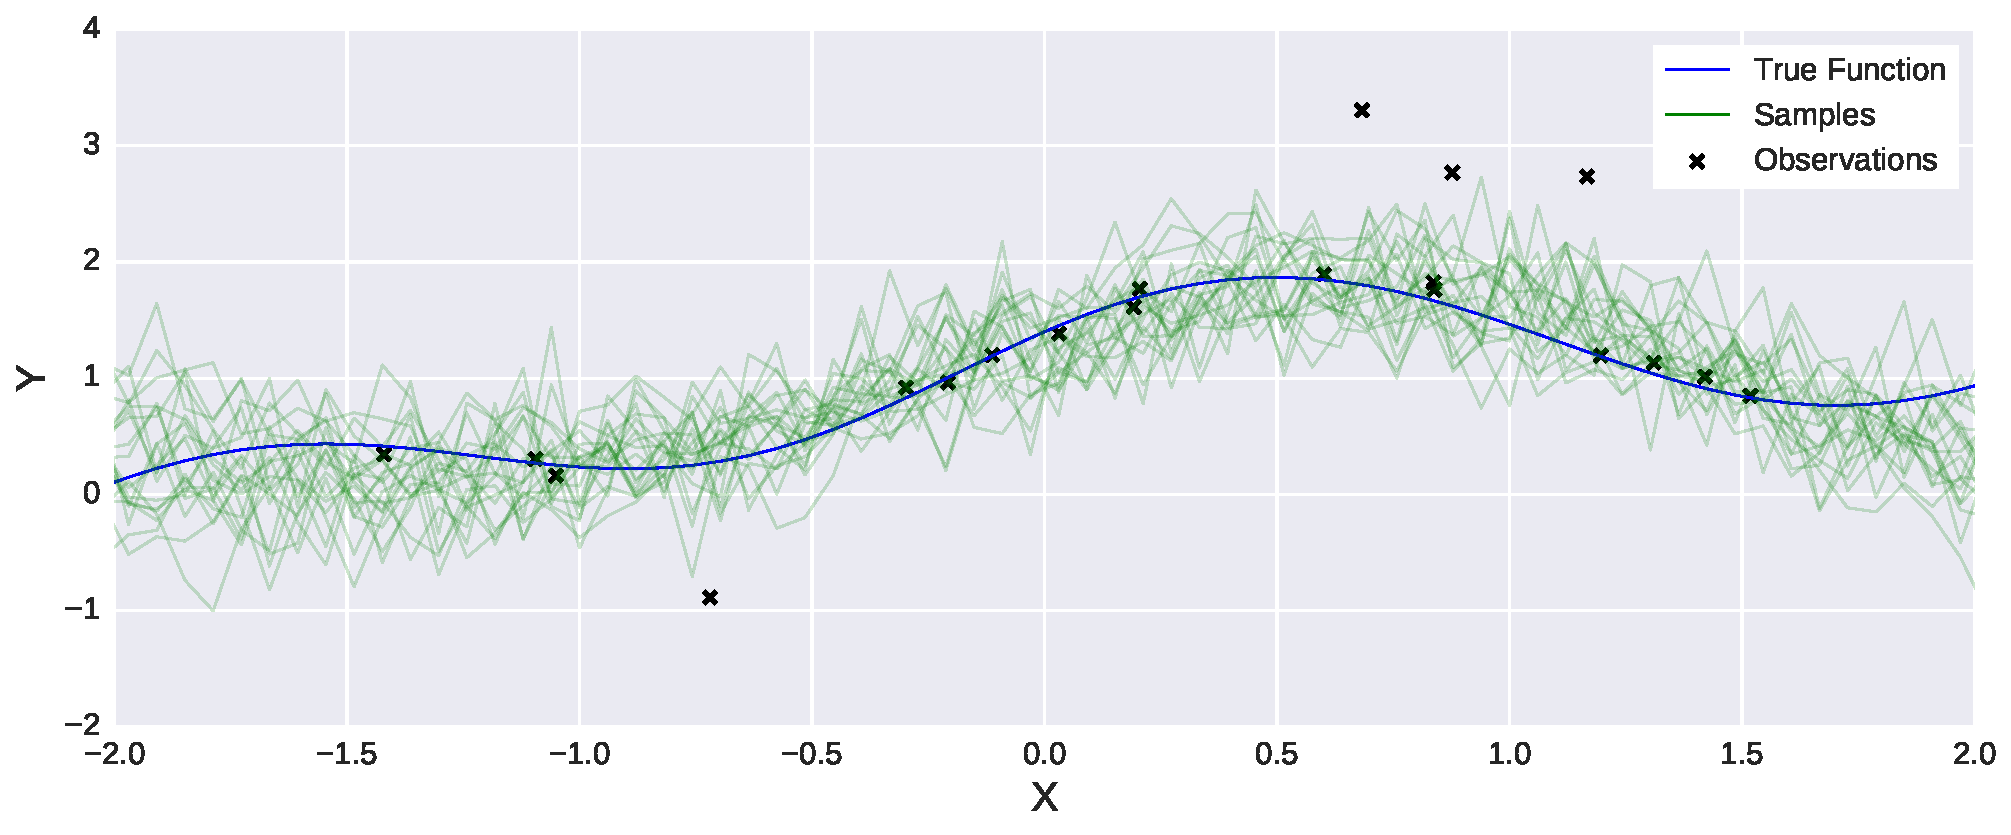
\includegraphics[width=0.85\textwidth]{figs/revised_figures/neal/predictive_posterior.pdf}
};
\node[below=4.5cm of e, yshift=0.0cm] (g) {(g)};
\node[above=-0.3cm of predictive_posterior, yshift=0.0cm]
(predictive_posterior_title) {\footnotesize Predictive posterior in the presence of outliers};



  % horizontal lines  
\node[right=\lineLength of a.north west] (a_helper) {};
\node[right=\lineLength of b.north west] (b_helper) {};
\node[right=\lineLength of c.north west] (c_helper) {};
\node[right=\lineLength of d.north west] (d_helper) {};
\node[right=\lineLength of e.north west] (e_helper) {};
\node[right=\lineLength of g.north west] (g_helper) {};
  \draw[shorten <=\shortenLine] 
    (a.north east) -- (a_helper); 
  \draw[shorten <=\shortenLine] 
    (b.north east) -- (b_helper); 
  \draw[shorten <=\shortenLine] 
    (c.north east) -- (c_helper); 
  \draw[shorten <=\shortenLine] 
    (d.north east) -- (d_helper); 
  \draw[shorten <=\shortenLine] 
    (e.north east) -- (e_helper); 
  \draw[shorten <=\shortenLine] 
    (g.north east) -- (g_helper); 
\end{tikzpicture}
